\section{Inovações e contribuições}
\label{sec:resultados}

\subsection{Contribuições científicas, tecnológicas e inovação}
O presente projeto também tem o objetivo de desenvolver pesquisas aplicada na área de Engenharia de Software,
Ciências da Computação e pesquisas em aprendizado de máquina, devops, engenharia de software contínua.

Como apresentado nos objetivos e escopo do projeto, o objetivo é pesquisar
formas de desenvolver e evoluir tecnologias livres, acesso livre à informação, e participação social na
gestão pública, no contexto das leis de incentivo a cultura, via o Ministério. O uso
software livre e uso de metodologias ágeis para o seu desenvolvimento
fortalecem institucionalmente o Ministério da Cultura, além de contribuir indiretamente com a plataforma de tecnológica de administração
pública.  

Técnicas de aprendizado de máquina frequentemente envolvem um elevado grau de formalismo matemático associado ao empirismo e 
intuição na montagem e calibração dos algoritmos utilizados. Esperamos obter não só avanços teóricos no sentido de encontrar 
soluções e aprimoramentos para os algoritmos para auxílio da plataforma SALIC, como também obter insumos para a análise 
quantitativa da performance dos métodos considerando tanto o ponto de vista de eficiência computacional quanto o da qualidade dos 
resultados obtidos. O objetivo nesta etapa consiste em explorar aprimoramentos de eficácia computacional e implementação de estratégias de treinamento online que viabilizem a análise de grandes volumes de dados em tempo real.

% O processo de desenvolvimento é um elemento-chave na produção de software, podendo ser responsável direto pela qualidade do produto gerado. 
% O requisito de se utilizar softwares livres associados a estratégias de governança digital exige uma customização nos processos de desenvolvimento de software. Exigirá também uma investigação de boas práticas em comunidades onde o Estado participa por adesão, possibilitando um ciclo de aprendizado na equipe do Ministério. Em particular, investigaremos como modelos de referência baseados em metodologias ágeis poderão ser adaptados para uso neste projeto.

A abordagem metodológica para a produção de software a ser empregada no projeto é prioritariamente de natureza empírica, aplicada e de design.
A natureza empírica decorre principalmente do foco do projeto na construção de soluções inovadoras aplicadas ao mundo real, adotando o ferramental
e metodologias consagradas pelo uso em comunidades de software livre. O ciclo de trabalho adotado pelo LAPPIS contempla o constante desenvolvimento
e evolução de software, onde os métodos empregados são continuamente refinados e re-analisados na forma de uma metodologia do tipo Pesquisa-Ação. 
Finalmente, a abordagem também contempla o design já que também almeja produzir artefatos sob a forma de documentação e de um guia metodológico. 

A inovação tecnológica poderá ser observada em:

\begin{itemize}
 \item Documentação e guia metodológico desenvolvidos 	para adoção da arquitetura de uma plataforma livre (lincença, ferramentas, documentação).
 
 \item Relatórios técnicos e documentação. Além da documentação técnica,  de grande importância para a comunidade de software livre, 
 espera-se ao final desse projeto a publicação de artigos em conferências/periódicos Qualis em Engenharia de software com os principais 
 resultados encontrados na pesquisa da metodologia ágil e Devops no contexto de software livre,
 e nas pesquisas em  aprendizado de máquina aplicadas à Plataforma de SALIC.
 
 \item Software desenvolvidos pelo projeto sob licença de software livre. 
 As principais inovações no desenvolvimento de software esperados no projeto são a desenvolvimento dos seguintes sistemas:
 \begin{itemize}
  \item \textit{Catálogo de Software} - plataforma para disponibilizar as diversas soluções informatizadas utilizadas  pelo Ministério da
 Cultura. O catálogo será desenvolvido segundo as práticas mais modernas de engenharia de software e é uma ferramenta que promove visibilidade
 do portfólio de produtos de softwares desenvolvidos por uma instituição. Será desenvolvido como software livre, 
 e pode ser utilizado para outras instituições, inclusive pela Universidade de Brasília.
  
  \item \textit{SIMEC frontend} - Incorporar boas práticas e tecnologias recentes ao software legado SIMEC, por meio de técnicas de refatoração
  de código legado. A inovação será no desacoplamento do frontend com o backend, documentação do projeto, e disponibilização como código aberto,
  de forma a facilitar a contribuição de desenvolvedores da comunidade de software livre. 

  
   \item \textit{Astromech} - Biblioteca de Machine Learning. A inovação é a integração de  funcionalidades de diversas bibliotecas
  abertas para esse fim, tais como scikit-learn\footnote{\url{ http://scikit-learn.org}}, tensorflow\footnote{\url{https://www.tensorflow.org/}}, 
  gensim\footnote{\url{https://radimrehurek.com/gensim/}}, nltk\footnote{\url{http://www.nltk.org/}}, 
  TextBlob\footnote{\url{https://textblob.readthedocs.io/en/dev/}} e matplotlib\footnote{\url{ https://matplotlib.org/}}.
  
  \item \textit{Astromech Django} - Wrapper de Integração do Astromech a ser desenvolvido com o framework Django.  A inovação principal é facilitar 
  para desenvolvedores de sistemas web com o framework django o uso de técnicas de aprendizado de máquina.
  
  \item \textit{Microserviço SALIC Data} - Microserviço que realiza a mineração dos dados dos projetos submetidos por meio da plataforma SALIC 
  e aplica técnicas de machine learning para extração de padrão, detecção de anomalias. A inovação principal 
  
  \item \textit{Chatbot} - software de assistentes virtuais (agentes virtuais) que trabalha e gerencia as trocas de mensagens, desenvolvido
  no contexto para tirar dúvidas dos proponentes de projetos via Lei Rouanet. Serão aplicados técnicas de processamento de linguagem natural (em
  lingua portuguesa), técnicas de aprendizado de máquina (árvores de decisão). Todo software será disponibilizado como software livre, 
  possibilitando o reuso das funcionalidades em diferentes contextos.
%   robot, rocket chat
  
  \item \textit{Jarbas} - projeto de gestão e configuração para automatizar tarefas de devops desenvolvido em python. 
 \end{itemize}

\end{itemize}

% \begin{itemize}

% Estudos da aplicação de metodologias ágeis e prática devops no processo de evolução de software.
% 
% \item Estudo de técnicas de aprendizado de máquina e processamento de linguagem natural.
% 
% \item Publicação dos principais resultados encontrados, e contribuições para a comunidade científica.
% 
% \item Softwares desenvolvidos com licenças livres, para acesso de toda a comunidade acadêmica, podendo ser reutilizado
% pela própria Universidade de Brasília.
% 
% \item Relatórios técnicos com os principais resultados encontrados.

% \end{itemize}
% 
% \subsection{Tecnológicos}
% 
% \begin{itemize}
% 
% \item Levantamento das ferramentas, práticas, e inovações da comunidade de software livre.
% 
% \item Protótipos e guias de utilização das ferramentas desenvolvidas.
% 
% \item Estudo de técnicas de aprendizado de máquina e processamento de linguagens naturais.
% 
% \item Relatórios técnicos e documentação.
% 
% \end{itemize}

\subsection{Contribuições Acadêmicas, Econômicas e Sociais}

 É importante ressaltar que o LAPPIS atualmente envolve cerca de 30 alunos em diversos
estágios de formação no curso de Engenharia de Software e que o presente projeto envolverá a maior parte destes alunos, quer seja em um ciclo 
de formação e desenvolvimento, quer seja em na forma de trabalhos de conclusão de curso para os alunos veteranos.

O curso de Engenharia de Software no Gama não possui um programa de pós-graduação e, portanto, a estratégia do LAPPIS se foca principalmente na 
formação de alunos de graduação por meio de envolvimento em questões práticas de desenvolvimento em projetos de software livre. O LAPPIS possui
uma parceria estratégica com o CCSL do IME-USP, onde vários ex-alunos são encaminhados para a pós-graduação e continuam mantendo um vínculo com 
projetos que envolvem alunos e professores do laboratório.

Além disto, o projeto envolve diretamente, como equipe do projeto, pelo menos um membro do programa de doutorado da COPPE-UFRJ
(linha de pesquisa sobre Experimentação Contínua e Mineração em Repositórios de Software) e produzirá material empírico rico para pesquisas
sobre  aferição de qualidade produto de software para a Administração Pública Federal, utilizando inicialmente o contexto do Ministério da
Cultura para a realização de pesquisa teórico-prática.

A proposta de que toda a pesquisa e desenvolvimento seja realizados como software livre, promove o desenvolvimento colaborativo junta as
soluções propostas por diferentes atores em um único repositório, gerando uma economia não estimada em relação à duplicação de esforços.  
As contribuições individuais de cada desenvolvedor são apresentadas de forma transparente em repositórios abertos, dado assim 
visibilidade das competências técnicas dos alunos.

Adicionalmente, serão produzidas algumas sistematizações relacionadas aos mecanismos de governança digital para co-produção de tecnologias e políticas em conjunto com as comunidades de software livre que o Estado participa por adesão. Esse material, além de subsidiar as estratégias de comunicação e ativação em torno da gestão do catálogo de software, também irão proporcionar publicações e repositórios úteis para a área de pesquisa da governança digital, normalmente relacionada às ciências sociais, ciência política e gestão pública.

%  Colaboração do Ministério com um laboratório de pesquisa como núcleo de pesquisa e desenvolvimento
%  de tecnologias inovadoras para políticas públicas do Ministério da Cultura.


\section{Vigência}

Este projeto terá a vigência de 24 (vinte e quatro) meses, posteriormente a sua data de
assinatura.

Na Figura \ref{figura-cronograma} é apresentada uma visão geral das atividades ao
longo do tempo, conforme os itens apresentados na EAP. O 
início das atividades está condicionado à confirmação do cronograma de desembolso
financeiro apresentado na secção \ref{sec:orcamento}.

%-------------------------------------------------------------------------------
% \begin{landscape}






%-------------------------------------------------------------------------------
% \newpage
 
%-------------------------------------------------------------------------------
\newpage
\section{Orçamento}
\label{sec:orcamento}

% Sugiro tirar essa parte já que teremos o detalhamento na planilha de custo

A maior parte dos recursos previstos no projeto são bolsas para pesquisa e 
desenvolvimento em Engenharia de Software. Os principais aquisições de recursos 
materiais são:

\begin{itemize}
\item \textbf{Contêiner}: está previsto a compra de cerca de 4 contêiners habitávies e mobiliário 
  para compor o espaço físico do LAPPIS. Este espaço adicional é necessário para
  acomodar a equipe do projeto e criar um laboratório de desenvolvimento que 
  comporte todos os membros envolvidos. A metodologia de desenvolvimento empregada
  no LAPPIS pressupõe encontros presenciais e que a equipe esteja frequentemente
  reunida.
\item \textbf{Material de Consumo}: está previsto a compra de material de 
  consumo para ser utilizado no laboratório.
\item \textbf{Viagens e Diárias}: está previsto gasto em passagens e diárias 
  para viabilizar o translado de parte da equipe em eventuais participações em 
  congressos e encontros em comunidades de software livre do portifólio MinC. 
\end{itemize}

Este Projeto está formalmente concebido como Projeto colaborativo no contexto de um Termo de Execução Descentralizada intra Governo Federal.
Essa característica faz com que a natureza de execução, além da relação entre as partes se dê de forma diferenciada daquela de contratos comerciais.
Neste contexto, o dimensionamento do Projeto possui como base o Programa de bolsas de pesquisa da UnB que é similar aos programas do MCTIC/FINEP  e
MEC/CAPES. Desta forma, o dimensionamento é feito pelo quantitativo de pesquisadores, estudantes e/ou profissionais que são necessários ao projeto e 
da especificação do perfil adequado à bolsa, respeitando a composição da equipe da UnB, preferencialmente, por pelo menos 60\% 
de integrantes do próprio quadro, entre professores pesquisadores e alunos. Todas as aquisições no âmbito do projeto serão precedidas dos componentes
licitatórios, na forma das Leis 8.666/1993 e 10.520/2002.
 
Abaixo detalhamos os recursos necessários para o desenvolvimento do Projeto, lembrando que os critérios para enquadramento e concessão de
Auxílio Financeiro à Pesquisador está de acordo com a Resolução do Conselho de Administração nº 0002/2012, que estabelece as normas para
pagamento de auxílio financeiro a estudante e pesquisador na forma de bolsas de estudo, pesquisa e extensão e a Lei nº 13.243 de 11 de janeiro de 2016.
Ainda, os critérios de enquadramento nas categorias e modalidades de bolsas, constantes do Programa de Apoio à Pesquisa, Desenvolvimento e Inovação 
– PPDI e descritos no Plano de Trabalho, bem como os valores a serem pagos (mínimo/máximo), estão condicionados à análise dos currículos Lattes 
pelo Núcleo de Recursos Humanos do CDT/FUB, que avalia a qualificação e experiência do candidato à bolsa. Outros critérios também são analisados 
pelo Coordenador como carga horária dedicada ao projeto e complexidade da atividade a ser realizada (a carga horária varia de 20 à 30 horas semanais).
 
A seleção dos bolsistas é da responsabilidade do Coordenador do Projeto observando o disposto nas chamadas públicas para seleção de profissionais 
vinculada ao Plano de Trabalho estabelecido, assim como é de responsabilidade do CDT/UnB a correta utilização dos recursos disponibilizados para
as finalidades previstas no Projeto.
 
\begin{itemize}
 \item Modalidade de Bolsa: \textbf{Pesquisador Sênior}
  Descrição: Pesquisador com experiência superior a quatro anos na coordenação executiva e execução de projetos de pesquisa e/ou implantação
  de processos gerenciais
  \begin{enumerate}
   \item   Nível A
   
Critérios de Enquadramento: Profissional com qualificação e experiência de pelo menos 8 (oito) anos na coordenação de projetos de P, 
D\&I e/ou em implantação de processos gerenciais
Valor Mensal: $5.501,00$ até $7.500,00$.
  \item  Nível B
Critérios de Enquadramento: Profissional com qualificação e experiência de pelo menos 6 (seis) anos na coordenação de projetos de P,
D\&I e/ou em implantação de processos gerenciais
Valor Mensal: $4.201,00$ até $5.500,00$.
  \end{enumerate}

   \item Modalidade de Bolsa: \textbf{Pesquisa, Desenvolvimento e Inovação PDI}
Descrição: Execução de projetos de pesquisa voltados ao desenvolvimento tecnológicos e inovação
  \begin{itemize}
   \item  Nível C
Critérios de Enquadramento: Profissional com qualificação e experiência de pelo menos 2 (dois) anos em projetos de P, D\&I e/ou em implantação
de processos gerenciais
Valor Mensal: $2.201,00$ até $3.200,00$.
  \end{itemize}
  \item Modalidade de Bolsa: \textbf{Apoio Técnico à Pesquisa}
Descrição: Execução de atividades de apoio técnico e/ou de apoio operacional à pesquisa, bem como atividades de extensão ligadas à pesquisa.
  \begin{itemize}
   \item  Nível A
Critérios de Enquadramento: Profissional que possuam experiência e conhecimentos técnicos necessários para a execução das atividades de pesquisa e de extensão de projetos cuja complexidade exija tal perfil profissional.
Valor Mensal: $801,00$ até $1.800,00$.
  \end{itemize}

\end{itemize}
  
 
Abaixo detalhamos os recursos necessários para o desenvolvimento do projeto,
lembrando que os mesmos serão objetos de constantes análises a serem discutidas
entre os envolvidos.

\begin{table}[!htb]
\rowcolors{3}{lightgray}{white}
\input{tabelas/bolsas2017.ltx}

\caption{Auxílio-Financeiro a Pesquisadores}
\label{tabela-bolsas}

\end{table}


\begin{table}[!htb]
\rowcolors{3}{lightgray}{white}
\input{tabelas/PessoaJuridica.ltx}
\caption{Outros Serviços de
Terceiros - Pessoa Jurídica.}
\label{tabela-PJ}
\end{table}

\begin{table}[!htb]
\rowcolors{3}{lightgray}{white}
\input{tabelas/material-consumo.ltx}
\caption{Material de Consumo.}
\label{tabela-consumo}
\end{table}

\begin{table}[!htb]
\rowcolors{3}{lightgray}{white}
\input{tabelas/material-permanente.ltx}
\caption{Serviços de Terceiros Pessoa Jurídica.}
\label{tabela-mat-permanente}
\end{table}
% \footnotetext{Nos termos do art. 12A, VI do Decreto 6.170/2007 
%   e da Resolução do Conselho de Adminsitração - CAD-UnB Nº 0045/2014}
%   
\begin{table}[!htb]
\rowcolors{3}{lightgray}{white}
\input{tabelas/passagens.ltx}
\caption{Passagens e Despesas com Locomoção.}
\label{tabela-passagens}
\end{table}


\begin{table}[!htb]
\rowcolors{3}{lightgray}{white}
\input{tabelas/diarias.ltx}
\caption{Diárias Pessoal Civil.}
\label{tabela-diarias}
\end{table}

\begin{table}[!htb]
\rowcolors{3}{lightgray}{white}
\input{tabelas/container.ltx}
\caption{ Equipamentos e Material Permanente}
\label{tabela-container}
\end{table}



\begin{table}[!htb]
\rowcolors{3}{lightgray}{white}
\input{tabelas/consolidado.ltx}
\caption{Orçamento consolidado}
\label{tabela-orcamento-consolidado}
\end{table}


O CDT/UnB, unidade da Universidade de Brasília, responsável pela administração
do projeto, trabalha com um conjunto de pesquisadores, inclusive de outras
áreas de conhecimento, e tem histórico de projetos de Desenvolvimento \&
Pesquisa, via o laboratório LAPPIS, da UnB Gama.
%
As fontes orçamentária estão conforme apresentados na Tabela
 \ref{tabela-bolsas}. 
%
As equipes da UnB trabalharão nas atividades conforme a proposta da Estrutura
Analítica do Projeto (EAP).

%-------------------------------------------------------------------------------
\newpage
\section{Cronograma de desembolso financeiro}
\label{sec:financeiro}

A descentralização orçamentária será feita  na UG/Gestão Recebedora: 
154019/15257– Fundação Universidade de Brasília/Centro de Apoio ao 
Desenvolvimento Tecnológico (CDT/FUB), com previsão orçamentária de $
 R\$2.078.600,00$ (Dois milhões, setenta e oito mil, e seiscentos reais).
 Na assinatura do Termo de descentralização, e a cada três meses serão feitos repasses, mediante
 a apresentação de relatórios de acompanhamento. Os valores de cada repasse estão detalhados
 na Tabela \ref{tabela-desembolso}.
\begin{landscape}
\begin{table}[!htb]
\rowcolors{3}{lightgray}{white}
 \input{tabelas/cronograma-desembolso.ltx}
\caption{Cronograma de desembolso financeiro.}
\label{tabela-desembolso}
\end{table}
\end{landscape}
\section{Cronograma de execução}
\label{sec:cronograma}

\begin{figure}[!htb]
\centering
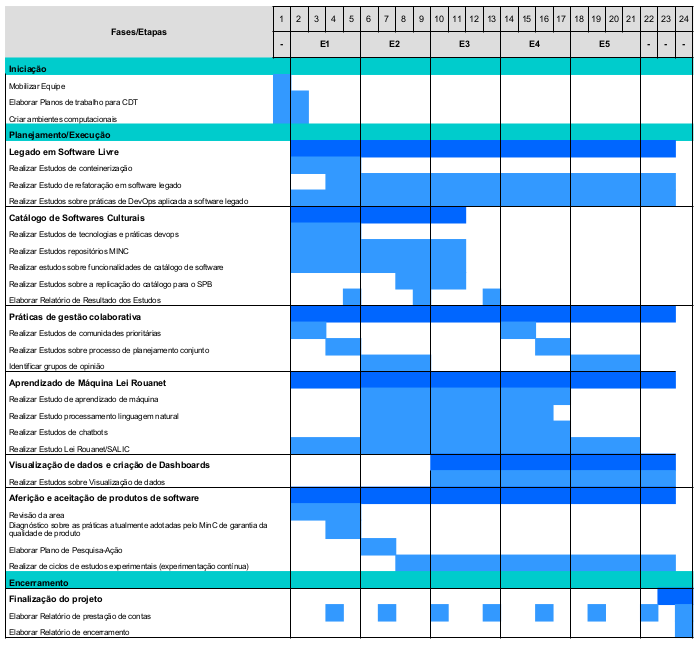
\includegraphics[scale=0.65]{figuras/Cronograma-LAPPIS-MINC.png}
\caption{Cronograma geral de atividades.}
\label{figura-cronograma}
\end{figure}
% \end{landscape}

